\documentclass[12pt]{report}
\usepackage[font=small, labelfont=bf]{caption}
\usepackage[english]{babel}
\usepackage{sectsty}
\usepackage{float}
\usepackage{amsmath}
\usepackage{amssymb}
\usepackage{siunitx}

\usepackage{graphicx} % For plots

%%% Custom Settings %%%
\setcounter{tocdepth}{3}                            % Include subsubsections in ToC
\setcounter{secnumdepth}{3}
\sisetup{mode=text,range-phrase = {\text{~to~}}}    % Change range ( atob -> a to b )
\newcommand\tab[1][1cm]{\hspace*{#1}}               % Use tabs
\newcommand{\dd}[1]{\mathrm{d}#1}                   % Integral's dd
\newcommand{\abs}[1]{\lvert #1 \rvert}              % Defines an abs() function
\newcommand{\overbar}[1]{\mkern 1.5mu\overline{\mkern-1.5mu#1\mkern-1.5mu}\mkern 1.5mu} % Defines a larger bar
\newcommand{\viff}{\Big\Updownarrow}                % Vertical iff()

\title{ \normalsize \LARGE {\uppercase{Communication Theory Homework 5}}}
\author{
    Derek Lee \\\\ 
    Professor Frost \\ ECE-300 \\ Communication Theory
}
\date{\today}

\begin{document}

\maketitle
\newpage

%%%%%%%%%%%%%%%%%%%%%%%%%%%%%%%%%%%%%%%%%%%% ADD THEOREM AND FIGURE
\section*{Question 1}
\textit{Describe when and why we use raised cosine pulses, citing the necessary conditions, at least
one theorem and drawing at least one figure.} \\

We use raised cosine pulses to reduce the probability of intersymbol interference (ISI) occurring. \\

\begin{figure}[H]
    \begin{equation}
        x(nT) =
        \begin{cases}
            1, & n = 0 \\
            0, & n \neq 0 
        \end{cases} \\
    \end{equation} \\
    
    \centering \viff
    
    \begin{equation}
        \sum_{m=-\infty}^{\infty} X(w+\frac{2\pi m}{T}) = T
    \end{equation}
    \caption{Nyquist Criterion for Zero ISI}
\end{figure}
    
    
\begin{equation}
    X_{rc}(w) =
    \begin{cases} 
        T, & 0 \leq \abs{w} \leq \pi \frac{(1-\alpha)}{T} \\
        \frac{T}{2}(1+\cos(\frac{T}{2\alpha}( \abs{w} - \pi \frac{(1-\alpha)}{T} ))), & \pi \frac{(1-\alpha)}{T} \leq \abs{w} \leq \pi \frac{(1+\alpha)}{T} \\
        0, & \abs{w} > \pi \frac{(1+\alpha)}{T}
    \end{cases}
\end{equation} 

\begin{figure}[H]
    \begin{center}
        \includegraphics[scale=1]{raisedCos.eps}
        \caption{Raised cosine generated with MATLAB}
    \end{center}
\end{figure}

$\alpha$ is the ``rolloff factor", where $\alpha \in [0,1]$

%%%%%%%%%%%%%%%%%%%%%%%%%%%%%%%%%%%%%%%%%%%%
\section*{Question 2}
\textit{True raised cosine pulses are not realizable – why not? What is done in practice to approximate
the raised cosine?} \\

True cosine pulses aren't realizable because they are infinite in time and they are non-causal.
They are approximated by truncating the signal and shifting in time by $t_o$, so they become finite in time and causal.

%%%%%%%%%%%%%%%%%%%%%%%%%%%%%%%%%%%%%%%%%%%%
\section*{Question 3}
\textit{Find the entropy of a geometrically distributed random variable (that is, a variable with
probability mass function $f(m) = p(1-p)^{m-1}$ for positive integer $m$ and some fixed probability $p$) as a function of $p$.}

\begin{figure}[H]
    \begin{gather}
        \displaystyle\sum_{k=0}^{\infty} r^k = \frac{1}{1-r} \\
        \displaystyle\sum_{k=0}^{\infty} k*r^{k-1} = \frac{1}{(1-r)^2} \label{Deriv}
    \end{gather}
    \caption{Taking the Derivative of the Geometric Series Formula}
\end{figure}


\begin{gather}
    H(p_i) = \displaystyle\sum_{i} -p_i \log(p_i) \\
    H(p) = \displaystyle\sum_{m=1}^{\infty} -p(1-p)^{m-1} \log(p(1-p)^{m-1}) \\
    = \displaystyle\sum_{m=0}^{\infty} -p(1-p)^{m} \log(p(1-p)^{m}) \\
    = \left[ -p \log(p) \displaystyle\sum_{m=0}^{\infty} \log(p(1-p)^{m}) \right] - 
            \left[ p \log(1-p) \displaystyle\sum_{m=0}^{\infty} m(1-p)^{m} \right] \\
    = \left[ -p \log(p) * \frac{1}{1-(1-p)} \right] - 
            \left[ p(1-p) \log(1-p) \displaystyle\sum_{m=0}^{\infty} m(1-p)^{m-1} \right] \\
    = \left[ -p \log(p) * \frac{1}{p} \right] - 
            \left[ p(1-p) \log(1-p) \displaystyle\sum_{m=0}^{\infty} m(1-p)^{m-1} \right] \\
    = -\log(p) - 
            \left[ p(1-p) \log(1-p) * \frac{1}{(1-(1-p))^2} \right] \quad 
            (\text{from \ref{Deriv}}) 
\end{gather}
\begin{gather}
    = -\log(p) - \left[ p(1-p) \log(1-p) * \frac{1}{p^2} \right] \\
    = -\log(p) - \frac{(1-p) \log(1-p)}{p}
\end{gather}

%%%%%%%%%%%%%%%%%%%%%%%%%%%%%%%%%%%%%%%%%%%%
\section*{Question 4}
\textit{Suppose a source has alphabet $\{ a_1, a_2, a_3, a_4, a_5, a_6, a_7, a_8 \}$ with corresponding output probabilities $\{ \frac{1}{16}, \frac{1}{16}, \frac{1}{4}, \frac{1}{32}, \frac{3}{32}, \frac{1}{8}, \frac{1}{16}, \frac{5}{16} \}$. Determine the entropy of the source.}

\begin{gather}
    H = \displaystyle\sum_{i} -p_i \log(p_i) \\
    H = 2.6258 \label{Huffman Entropy}
\end{gather}

\newpage

%%%%%%%%%%%%%%%%%%%%%%%%%%%%%%%%%%%%%%%%%%%%
\section*{Question 5}
\textit{Design a Huffman code for the above source. Validate that it satisfies the Kraft inequality,
and that the average length satisfies the Huffman code entropy inequalities.} \\

\begin{figure}[H]
    \begin{center}
        \includegraphics[scale=0.5]{Huffman.png}
        \caption{Huffman Coding}
    \end{center}
\end{figure}

\begin{table}[H]
    \centering
    \begin{tabular}{| c | c |} \hline
        Symbol & Encoding   \\ \hline
        $a_1$ & 1110        \\ \hline
        $a_2$ & 1011        \\ \hline
        $a_3$ & 01          \\ \hline
        $a_4$ & 1111        \\ \hline
        $a_5$ & 110         \\ \hline
        $a_6$ & 100         \\ \hline
        $a_7$ & 1010        \\ \hline
        $a_8$ & 00          \\ \hline
    \end{tabular}
    \caption{Codewords for each symbol}
    \label{tab:Huffman}
\end{table}

\begin{figure}[H]
    \begin{gather}
        \sum_{i=1}^{N} 2^{\ell_i} \leq 1 \\
        3*2^{-4} + 1*2^{-2} + 1*2^{-5} + 3*2^{-5} + 1*2^{-3} + 5*2^{-4} \leq 1 \\
        \frac{8}{16} + \frac{1}{4} + \frac{4}{32} + \frac{1}{8} \leq 1 \\
        \frac{1}{2} + \frac{1}{4} + \frac{1}{4} \leq 1 \\
        1 \leq 1 \ \checkmark
    \end{gather}
    \caption{Proof that the Huffman code satisfies the Kraft inequality}
\end{figure}

\begin{figure}[H]
    \begin{gather}
        \overbar{L} = 4p_1 + 4p_2 + 2p_3 + 4p_4 + 3p_5 + 3p_6 + 4p_7 + 2p_8 \\
        = \frac{1}{4} + \frac{1}{4} + \frac{1}{2} + \frac{1}{8} + \frac{9}{32} + \frac{3}{8} + \frac{1}{4} + \frac{5}{8} \\
        = 1 + \frac{3}{4} + \frac{29}{32} \\
        = 2.65625
    \end{gather}
    \begin{gather*}
        H = 2.6258 \quad 
        (\text{from \ref{Huffman Entropy}})
    \end{gather*}
    \begin{gather}
        H(x) \leq \overbar{L} \leq H(x) + 1 \\
        2.6258 \leq 2.65625 \leq 2.6258 + 1 \\
        2.6258 \leq 2.65625 \leq 3.6258 \ \checkmark
    \end{gather}
    \caption{Proof that the Huffman code satisfies the Huffman code entropy inequalities}
\end{figure}


%%%%%%%%%%%%%%%%%%%%%%%%%%%%%%%%%%%%%%%%%%%%
\section*{Question 6}
\textit{Find the transmission power (in Watts) necessary for an AWGN channel with $N_o$ = 108 J
and transmission bandwidth B = 1 MHz to achieve a channel capacity of 1 Mb/s.}

\begin{gather}
    C = W \log( 1 + \frac{P}{N_o W} ) \\
    P = N_o W( 2^{ \frac{C}{W} } - 1 ) \\
    P = 108MW
\end{gather}

\newpage

%%%%%%%%%%%%%%%%%%%%%%%%%%%%%%%%%%%%%%%%%%%%
\section*{Question 7}
\textit{The next several questions will refer to the (n,k) linear block code with generator matrix \\
    \begin{gather*}
        G =
        \left[ \begin{array}{ c c c c c c c }
                0 & 1 & 1 & 1 & 0 & 1 & 1 \\
                1 & 0 & 0 & 1 & 1 & 1 & 1 \\
                0 & 0 & 1 & 1 & 1 & 0 & 1 \\
        \end{array} \right]
    \end{gather*}
You may use MATLAB to help with any question below, although they can all be done by
hand. \\
First - What are n and k?}

\begin{equation}
    n = 7,\ k = 3
\end{equation}

%%%%%%%%%%%%%%%%%%%%%%%%%%%%%%%%%%%%%%%%%%%%
\section*{Question 8}
\textit{Make a list of every data vector and associated codeword.}

\begin{gather*}
    e_1 = (100) \rightarrow g_1 = (100)G = 0111011 \\
    e_2 = (010) \rightarrow g_2 = (010)G = 1001111 \\
    e_3 = (001) \rightarrow g_3 = (001)G = 0011101
\end{gather*}

% Write data vectors
\newcommand{\genDV}[3]{(#1*e_1) \oplus (#2*e_2) \oplus (#3*e_3) = (#1#2#3)}

\begin{figure}[H]
    \begin{gather*}
        x_0 = \genDV{0}{0}{0} \\
        x_1 = \genDV{0}{0}{1} \\
        x_2 = \genDV{0}{1}{0} \\ 
        x_3 = \genDV{0}{1}{1} \\
        x_4 = \genDV{1}{0}{0} \\
        x_5 = \genDV{1}{0}{1} \\
        x_6 = \genDV{1}{1}{0} \\
        x_7 = \genDV{1}{1}{1}
    \end{gather*}
    \caption{List of Data Vectors}
\end{figure}

% Write codewords
\newcommand{\genCW}[3]{(#1*g_1) \oplus (#2*g_2) \oplus (#3*g_3)}

\begin{figure}[H]
    \begin{gather*}
        C_0 = \genCW{0}{0}{0} = (0000000) \\
        C_1 = \genCW{0}{0}{1} = (0011101) \\
    	C_2 = \genCW{0}{1}{0} = (1001111) \\
    	C_3 = \genCW{0}{1}{1} = (1010010) \\
    	C_4 = \genCW{1}{0}{0} = (0111011) \\
    	C_5 = \genCW{1}{0}{1} = (0100110) \\
    	C_6 = \genCW{1}{1}{0} = (1110100) \\
    	C_7 = \genCW{1}{1}{1} = (1101001)
    \end{gather*}
    \caption{List of Codewords}
\end{figure}

%%%%%%%%%%%%%%%%%%%%%%%%%%%%%%%%%%%%%%%%%%%%
\section*{Question 9}
\textit{What is the minimum Hamming distance of the code, $d_{min}$? How many errors can this code
correct?} \\

\noindent The minimum Hamming distance is 3. 

\begin{gather}
    d(C) \geq 2k + 1 \\
    3 \geq 2k + 1 \\
    k \leq 1
\end{gather}

\noindent This code can correct at most 1 error.

\newpage

%%%%%%%%%%%%%%%%%%%%%%%%%%%%%%%%%%%%%%%%%%%%
\section*{Question 10}
\textit{There exists a systematic code with the same codewords as this code - how can you know
that from looking at the list? It should be straightforward to create the generator matrix of
this systematic code, $G_S$.} \\

\noindent Every non-systematic code can be transformed into a systematic code. 

\begin{gather}
    G_S = (I_k\ |\ P) \\
    G_S =  
    \left[ \begin{array}{ c c c | c c c c }
        1 & 0 & 0 & 1 & 1 & 1 & 1 \\
        0 & 1 & 0 & 0 & 1 & 1 & 0 \\
        0 & 0 & 1 & 1 & 1 & 0 & 1 \\
    \end{array} \right]
\end{gather}

%%%%%%%%%%%%%%%%%%%%%%%%%%%%%%%%%%%%%%%%%%%%
\section*{Question 11}
\textit{Find the parity check matrix of $G_S$, H.}

\begin{gather}
    H = (P^T\ |\ I_{n-k}) \\
    H = 
    \left[ \begin{array}{ c c c | c c c c }
        1 & 0 & 1 & 1 & 0 & 0 & 0 \\
        1 & 1 & 1 & 0 & 1 & 0 & 0 \\
        1 & 1 & 0 & 0 & 0 & 1 & 0 \\
        1 & 0 & 1 & 0 & 0 & 0 & 1 \\
    \end{array} \right]
\end{gather}

%%%%%%%%%%%%%%%%%%%%%%%%%%%%%%%%%%%%%%%%%%%%
\section*{Question 12}
\textit{Does H work as a parity check matrix for G? To help answer this, find GH and $G_S$H.} \\

The calculations are done in the associated MATLAB file.

\begin{gather}
    GH^T = 0\ \checkmark \\
    G_SH^T = 0\ \checkmark
\end{gather}

Yes, it works as a parity check matrix for G.

\end{document}